\documentclass[fleqn,10pt]{wlscirep}
\usepackage[utf8]{inputenc}
\usepackage[T1]{fontenc}
\usepackage{textcomp}
\usepackage{graphicx}
\usepackage{tablefootnote}
\usepackage{xr}

\makeatletter
\newcommand*{\addFileDependency}[1]{% argument=file name and extension
  \typeout{(#1)}
  \@addtofilelist{#1}
  \IfFileExists{#1}{}{\typeout{No file #1.}}
}
\makeatother


\newcommand*{\myexternaldocument}[1]{%
    \externaldocument{#1}%
    \addFileDependency{#1.tex}%
    \addFileDependency{#1.aux}%
}

\myexternaldocument{SI}

\title{NMRlipids Databank makes data-driven analysis of biomembrane properties accessible for all}
%NMRlipids Databank: Making data-driven analyses of membrane properties accessible for all^
%Overlay Databank of Lipid Membrane Simulations Arising from Open Collaboration

\author[1]{Anne Kiirikki}         %ORCID: ?
\author[2]{Hanne Antila}          %ORCID: 0000-0002-2474-5053
\author[2]{Lara Bort}             %ORCID: ?
\author[3]{Pavel Buslaev}         %ORCID: ?
\author[4]{Fernando Favela}
\author[5]{Tiago Mendes Ferreira}
\author[6,7]{Patrick Fuchs}
\author[8,9]{Rebeca Garcia-Fandino}
\author[2]{Ivan Gushchin}
%\author[2]{Matti Javanainen}      %ORCID: 0000-0003-4858-364X
\author[2]{Batuhan Kav}           %ORCID: ?
\author[2]{Milla Kurki}
\author[2]{Alexander Kuzmin}
\author[10,11]{Jesper Madsen}
\author[2]{Markus S. Miettinen}   %ORCID: 0000-0002-3999-4722
%\author[2]{...}                   %ORCID: ?
\author[12]{Thomas Piggot}
\author[2]{Suman Samantray}
\author[2]{Fabi{\'a}n Suarez-Leston}
\author[1,*]{O. H. Samuli Ollila} %ORCID: 0000-0002- 8728-1006
%\author[1,2,+]{Christine Author}
%\author[2,+]{Derek Author}

\affil[1]{University of Helsinki, Institute of Biotechnology, Helsinki, Finland}
\affil[2]{Affiliation, department, city, postcode, country}
\affil[3]{Nanoscience Center and Department of Chemistry, University of Jyv{\"a}skyl{\"a}, P.O. Box 35, Jyv{\"a}skyl{\"a}, 40014 , Finland}
\affil[4]{Departamento de Ciencias B\'{a}sicas, Tecnol\'{o}gico Nacional de M\'{e}xico - ITS Zacatecas Occidente, Sombrerete, Zacatecas, 99102, M\'{e}xico}
\affil[5]{NMR group - Institute for Physics, Martin Luther University Halle-Wittenberg,  Halle (Saale), 06120, Germany}
\affil[6]{Sorbonne Universit{\'e}, Ecole Normale Sup{\'e}rieure, PSL University, CNRS, Laboratoire des Biomol{\'e}cules (LBM), Paris, 75005, France}
\affil[7]{Universit{\'e} de Paris, UFR Sciences du Vivant, Paris, 75013, France}
\affil[8]{Center for Research in Biological Chemistry and Molecular Materials (CiQUS), Universidade de Santiago de Compostela,  Santiago de Compostela, E-15782, Spain}
\affil[9]{CIQUP, Centro de Investigação em Qu{\'i}mica, Departamento de Qu{\'i}mica e Bioqu{\'i}mica, Faculdade de Ci{\^e}ncias, Universidade do Porto, Porto, 4169-007, Portugal}
\affil[10]{Department of Chemistry, The University of Chicago, Chicago, Illinois, 60637, United States of America}
\affil[11]{Global and Planetary Health, College of Public Health, University of South Florida, Tampa, Florida, 33612, United States of America}
\affil[12]{Chemistry, University of Southampton, Highfield, Southampton, SO17 1BJ, United Kingdom}


\affil[*]{samuli.ollila@helsinki.fi}

%\affil[+]{these authors contributed equally to this work}

%\keywords{Keyword1, Keyword2, Keyword3}

\begin{abstract}
Cellular membrane lipid composition is implicated in diseases and major biological functions in cells, but membranes are difficult to study experimentally due to their intrinsic disorder and complex phase behaviour. Molecular dynamics (MD) simulations have been useful in understanding membrane systems, but they require significant computational resources and often suffer inaccuracies in model parameters. Applications of data-driven and machine learning methods, currently revolutionising many fields, are limited to membrane systems due to the lack of suitable training sets. Here we present the NMRlipids Databank---a community-driven, open-for-all database featuring programmatic access to quality evaluated atom-resolution MD simulations of lipid bilayers. The NMRlipids databank will benefit scientists in different disciplines by provoding automatic ranking of simulations based on their quality against experiments, flexible implementations of data-driven and machine learning applications, and rapid access to simulation data via graphical user interface. To demonstrate the unlocked possibilities beyond current MD simulation studies, we analyzed how anisotropic diffusion of water and cholesterol flip–flop rates depend on membrane properties.

\end{abstract}
\begin{document}

\flushbottom
\maketitle
% * <john.hammersley@gmail.com> 2015-02-09T12:07:31.197Z:
%
%  Click the title above to edit the author information and abstract
%
\thispagestyle{empty}

%\noindent Please note: Abbreviations should be introduced at the first mention in the main text – no abbreviations lists. Suggested structure of main text (not enforced) is provided below.

\section{Introduction}

%The demand for sharing and reusing of MD simulation data is increasing, but practical solution remains unclear due to unsolved issues in data storage and indexing.

Cellular membranes contain hundreds of different types of lipid molecules that regulate the membrane properties, morphology, and biological functions~\cite{vanmeer08,Lorent:2020a,Slatter:2016a}. Membrane lipid composition is implicated in diseases, such as cancer and neurodegenerative disorders, and therapeutics that affect membrane compositions are emerging~\cite{torres21}. However, biomembranes are often difficult to study experimentally because at biological conditions they are in disordered fluid state, and sample preparation can be arduous due to the complicated phase behaviour and rich interactions between lipids and other biomolecules. For those reasons, the detailed connections between complex lipid interactions and biological functions taking place in or around membranes remain poorly understood. Molecular dynamics (MD) simulations have been particularly useful in understanding membrane systems, although their accuracy has often been compromised by artefacts such as the quality of model parameters~\cite{antila22b,gupta22}. Presently, the accuracy of models is becoming increasingly important as researches are progressing from simulations of individual molecules to simulating whole organelles or even cells using interdisciplinary approaches~\cite{johnson15,thornburg22,gupta22}. Such systems exhibit complex emergent behaviour making inaccuracies more difficult to detect and accumulation of even modest errors may have major impact on the conclusions.

In contrast to experimental structural biology, where standard protocols to share and quality-evaluate the resolved structures are firmly established \textit{via} the Protein Data Bank (PDB)~\cite{montelione13}, the equivalent best practices are yet to be defined for MD simulations. The importance of such approaches is widely recognized~\cite{feig99,tai04,silva06,abraham19,hildebrand19,hospital20,abriata20,espigares20} and data-sharing solutions are emerging for proteins in solution~\cite{meyer10,kamp10}, proteins in membranes~\cite{newport19,espigares20,leston22}, nucleic acids~\cite{hospital16}, nucleic acids and proteins~\cite{bekker20}, cyclodextrins~\cite{mixcoha16}, COVID-19--involved macromolecules~(\url{bioexcel-cv19.bsc.es}). However, automatic quality evaluation of simulation data~\cite{meyer10,hospital16} and programmatic access is still rare. In particular, tools for automatic quality evaluation of membrane simulations, or training sets for machine learning models of membrane-containing systems, are not yet available. Recent advances using machine learning approaches utilizing publicly available databanks, for example to solve protein structures~\cite{jumper21}, emphasize the increasing importance of such resources. 
%The profound, and sometimes unexpected, effect that such open data sharing and quality evaluation can have on the field cannot be understated. At the very least, open access data will reduce the man and computational hours originating from double work, reducing the environmental impact. Beyond that, by providing the training data, the PDB laid the foundation for the machine learning algorithms now closing into solving the protein folding problem and the strides those machine learning tools have facilitated in the biomedical sciences since. 


Here we present the NMRlipids Databank---a community-driven, open-for-all database featuring programmatic access to atom-resolution MD simulations of lipid bilayers. The programmatic access enables users to apply data-driven approaches on the Databank, thus facilitating the creation of new tools for (and by) researchers in a wide range of fields covering academia and industry, from cell membrane biology and lipid nanoparticle formulations to computational chemistry and machine learning. As two usage examples of what is already possible, we demonstrate here (i) how data-driven analysis of water anisotropic diffusion in all the membrane systems available in the Databank can extend the scope of MD simulations to magnetic resonance imaging (MRI) and pharmacokinetics, and (ii) how the Databank allows its users to analyse rare phenomena that are beyond the scope of standard MD simulation investigations. Wider adaptation of the NMRlipids Databank will open even more possibities. Furthermore, the Databank performs automatic quality evaluation of membrane simulations, which facilitates the selection of best models for specific applications and accelerates the development of simulation parameters and methodology.  


While the NMRlipids Databank currently contains only lipid bilayer systems, it can readily be expanded to contain other molecules, such as disordered proteins or sugars. The powerful combination of the overlay databank structure and a community-wide open collaboration can be applied also when building databases in other fields, particularly when storage of raw data requires significant resources, best practices in the field are not defined, and incentives to share data do not exist. Therefore, the approach introduced here opens up possibilities to create databases enabling data-driven and machine learning applications in new fields.



\section{Results}

\subsection{Programmatic access to MD simulations of membranes composed of most common biologically abundant lipids}

NMRlipids Databank is a community-driven database containing atomistic MD simulations of biologically relevant lipid membranes emerging from the NMRlipids open collaboration~\cite{botan15,ollila16,catte16,antila19,bacle21}. It has been designed to improve data Findability, Accessibility, Interoperability, and Reuse (FAIR)~\cite{wilkinson16} using the NMRlipids project protocol where all the content is openly accessible from the beginning of the project~\cite{botan15}.  Currently the NMRlipids databank contains nearly thousand simulation trajectories with the total length approaching half a millisecond. The distribution of available simulations containing a specific lipid in Fig.~\ref{fig:overlay}C roughly resembles the biological abundance of different lipid types with phosphatidylcholine (PC) being the most common followed by cholesterol, phosphatidylethanolamine (PE), phosphatidylserine (PS), phosphatidylglycerol (PG), phosphatidylinositol (PI), and other lipids depending on organism and organelle~\cite{vanmeer08}. Currently available single component lipid membranes and binary mixtures in the NMRlipids databank are illustrated in Fig.~\ref{fig:overlay}D. While these comprise the majority of available trajectories, mixtures with up to five lipid types are available. Force fields used in simulations cover all the essential parameters commonly used in lipid simulations, see Fig.~\ref{fig:overlay}E, including also united atom and polarizable force fields. Therefore, the averages calculated over the databank can be considered as mean predictions from available lipid models for an average cell membrane.

The overlay structure, illustrated in Fig.~\ref{fig:overlay}A, is designed to enable efficient upcycling of MD simulations for data-driven and machine learning applications using 
The NMRlipids databank. Raw simulation data in the {\it data layer} can be stored in any publicly available location with long term stability, such as Zenodo (\url{zenodo.org}), and with permanent links to the data, such as digital object identifiers (DOIs). 
%or uniform resource names (URNs). 
The {\it Databank layer} is the core of the databank containing all the relevant information about the simulations, including links to the raw data, relevant metadata describing the systems, universal naming conventions for lipids and their atoms, computer programs to create and analyse the entries, basic properties calculated from all simulations (area per lipid, C--H bond order parameters, X-ray scattering form factors and membrane thickness), and quality evaluation of simulations against experimental data. In practise, this information is stored in the git repository which is available at~\url{https://github.com/NMRLipids/Databank}. The {\it application layer} contains outputs from the databank, such as graphical user interface (\url{http://www.databank.nmrlipids.fi/}) and results from analyses described in sections below which are available at \url{https://github.com/NMRLipids/DataBankManuscript}. A more detailed description on the NMRlipids databank structure is available the supplementary information. 



\begin{figure}
    \centering
    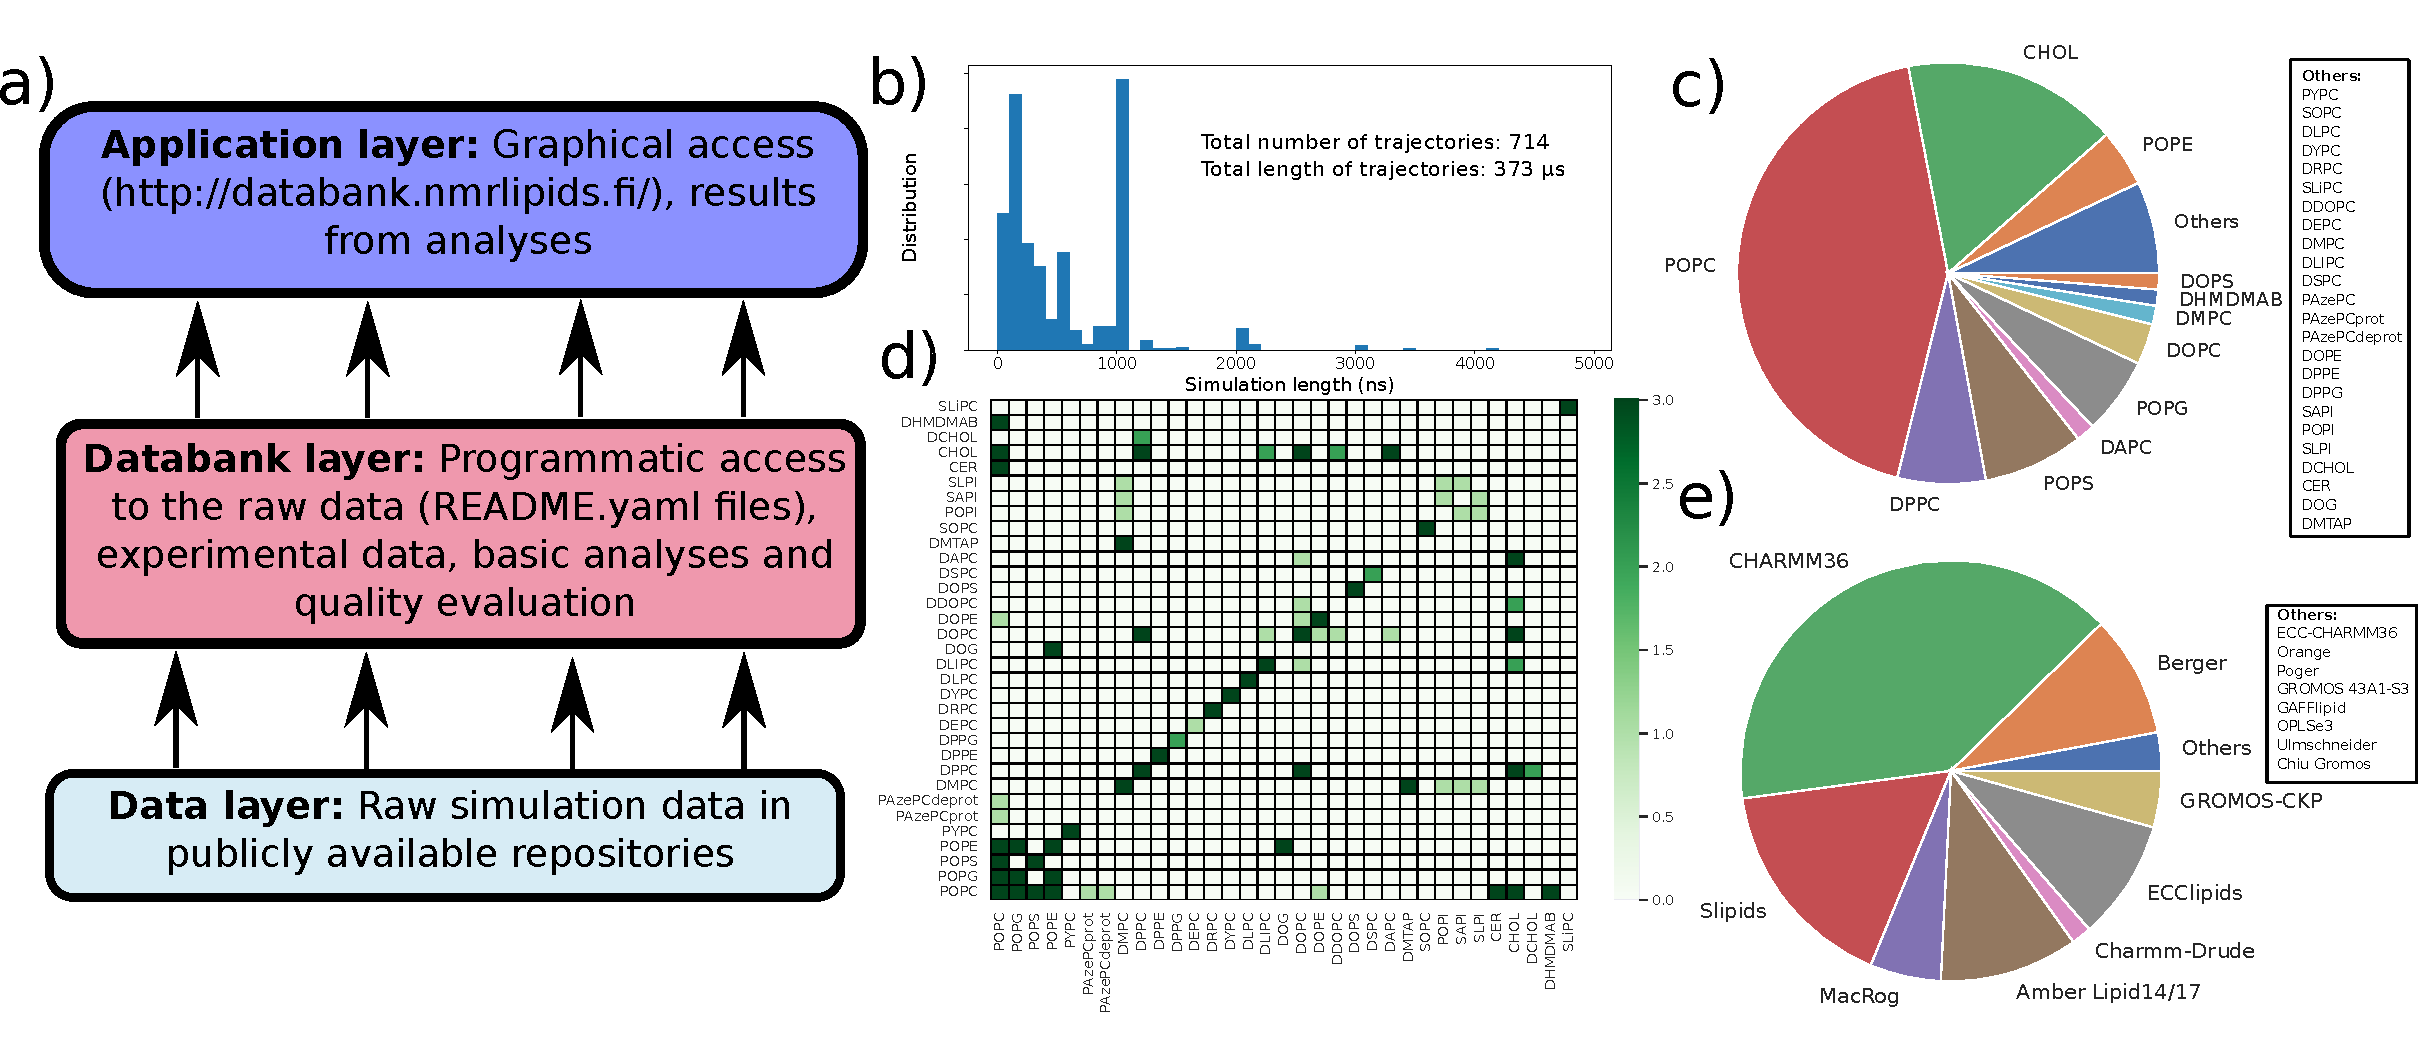
\includegraphics[width=\linewidth]{Figures/overlay2.pdf}
    \caption{a) Schematic presentation of the overlay structure used in the NMRlipids databank. A more detailed structure of the databank layer is shown in Fig.~\ref{DatabankStructure} in the SI.
    b) Distribution of the lengths of the trajectories, total number of trajectories and total length of the simulations in the NMRlipids databank.
    c) Distribution of lipids present in the trajectories in the NMRlipids databank. Lipids occuring in five or fewer simulations ('others') are listed on the right. 
    d) Currently available binary mixtures in the NMRlipids databank. 
    e) Distribution of force fields in the simulations in the NMRlipids databank.
    }
    \label{fig:overlay}
\end{figure}

\subsection{Accessing NMRlipids databank}\label{section:access}
The content of the NMRlipids databank is easily searchable and browsable via graphical user interface (GUI) (\url{http://www.databank.nmrlipids.fi/}), which can be also used to visualize the systems, compare basic properties between diffent systems and experiments, and rank simulations based on their quality evaluated against experimental data. 

%\subsection{Analyzing the databank}
More flexible analyses that enable wide range of novel applications can be performed by the Python application programming interface (API) available at \url{https://github.com/NMRLipids/Databank}. The API can be used to automatically analyse virtually any property from all simulations in the NMRlipids databank following the flowchart demonstrated in Fig.~\ref{fig:POPCPOPEapls}A. Iteration through the README.yaml files in the {\it databank layer} enables the access to raw simulation data via the links stored in these files. Affiliation of universal molecule and atom names to the simulation specific names in README.yaml and mapping files enable automatic analyses independently on the specific naming convention used in a simulation. Analysis codes and results for membrane area per lipid, C–H bond order parameters, X-ray scattering form factors and thickness are included in the {\it Databank layer}. Further analysis codes can be implemented by users and the results can be stored to the {\it application layer} in the same format that is used in the {\it Databank layer}. The results from analyses can be then programmatically accessed and furhter analyzed using the NMRlipids databank API following the flowchart demonstrated in Fig.~\ref{fig:POPCPOPEapls}B.

These tools offer open programmatic access to unprecedented amount of simulation trajectories for all, which enables possibilities for wide range of novel analyses. This is particularly useful for scientist without access to resources to perform large scale MD simulations and for analyses of rare phenomena that require exceptional amounts of simulation data. On the other hand, universal naming convention enables systematic comparisons between simulations having different model parameters and thereby different naming conventions. This will guide the development of more accurate simulation parameters and usage of atomistic models to train coarse grained simulations.

\begin{figure}[t]
    \centering
    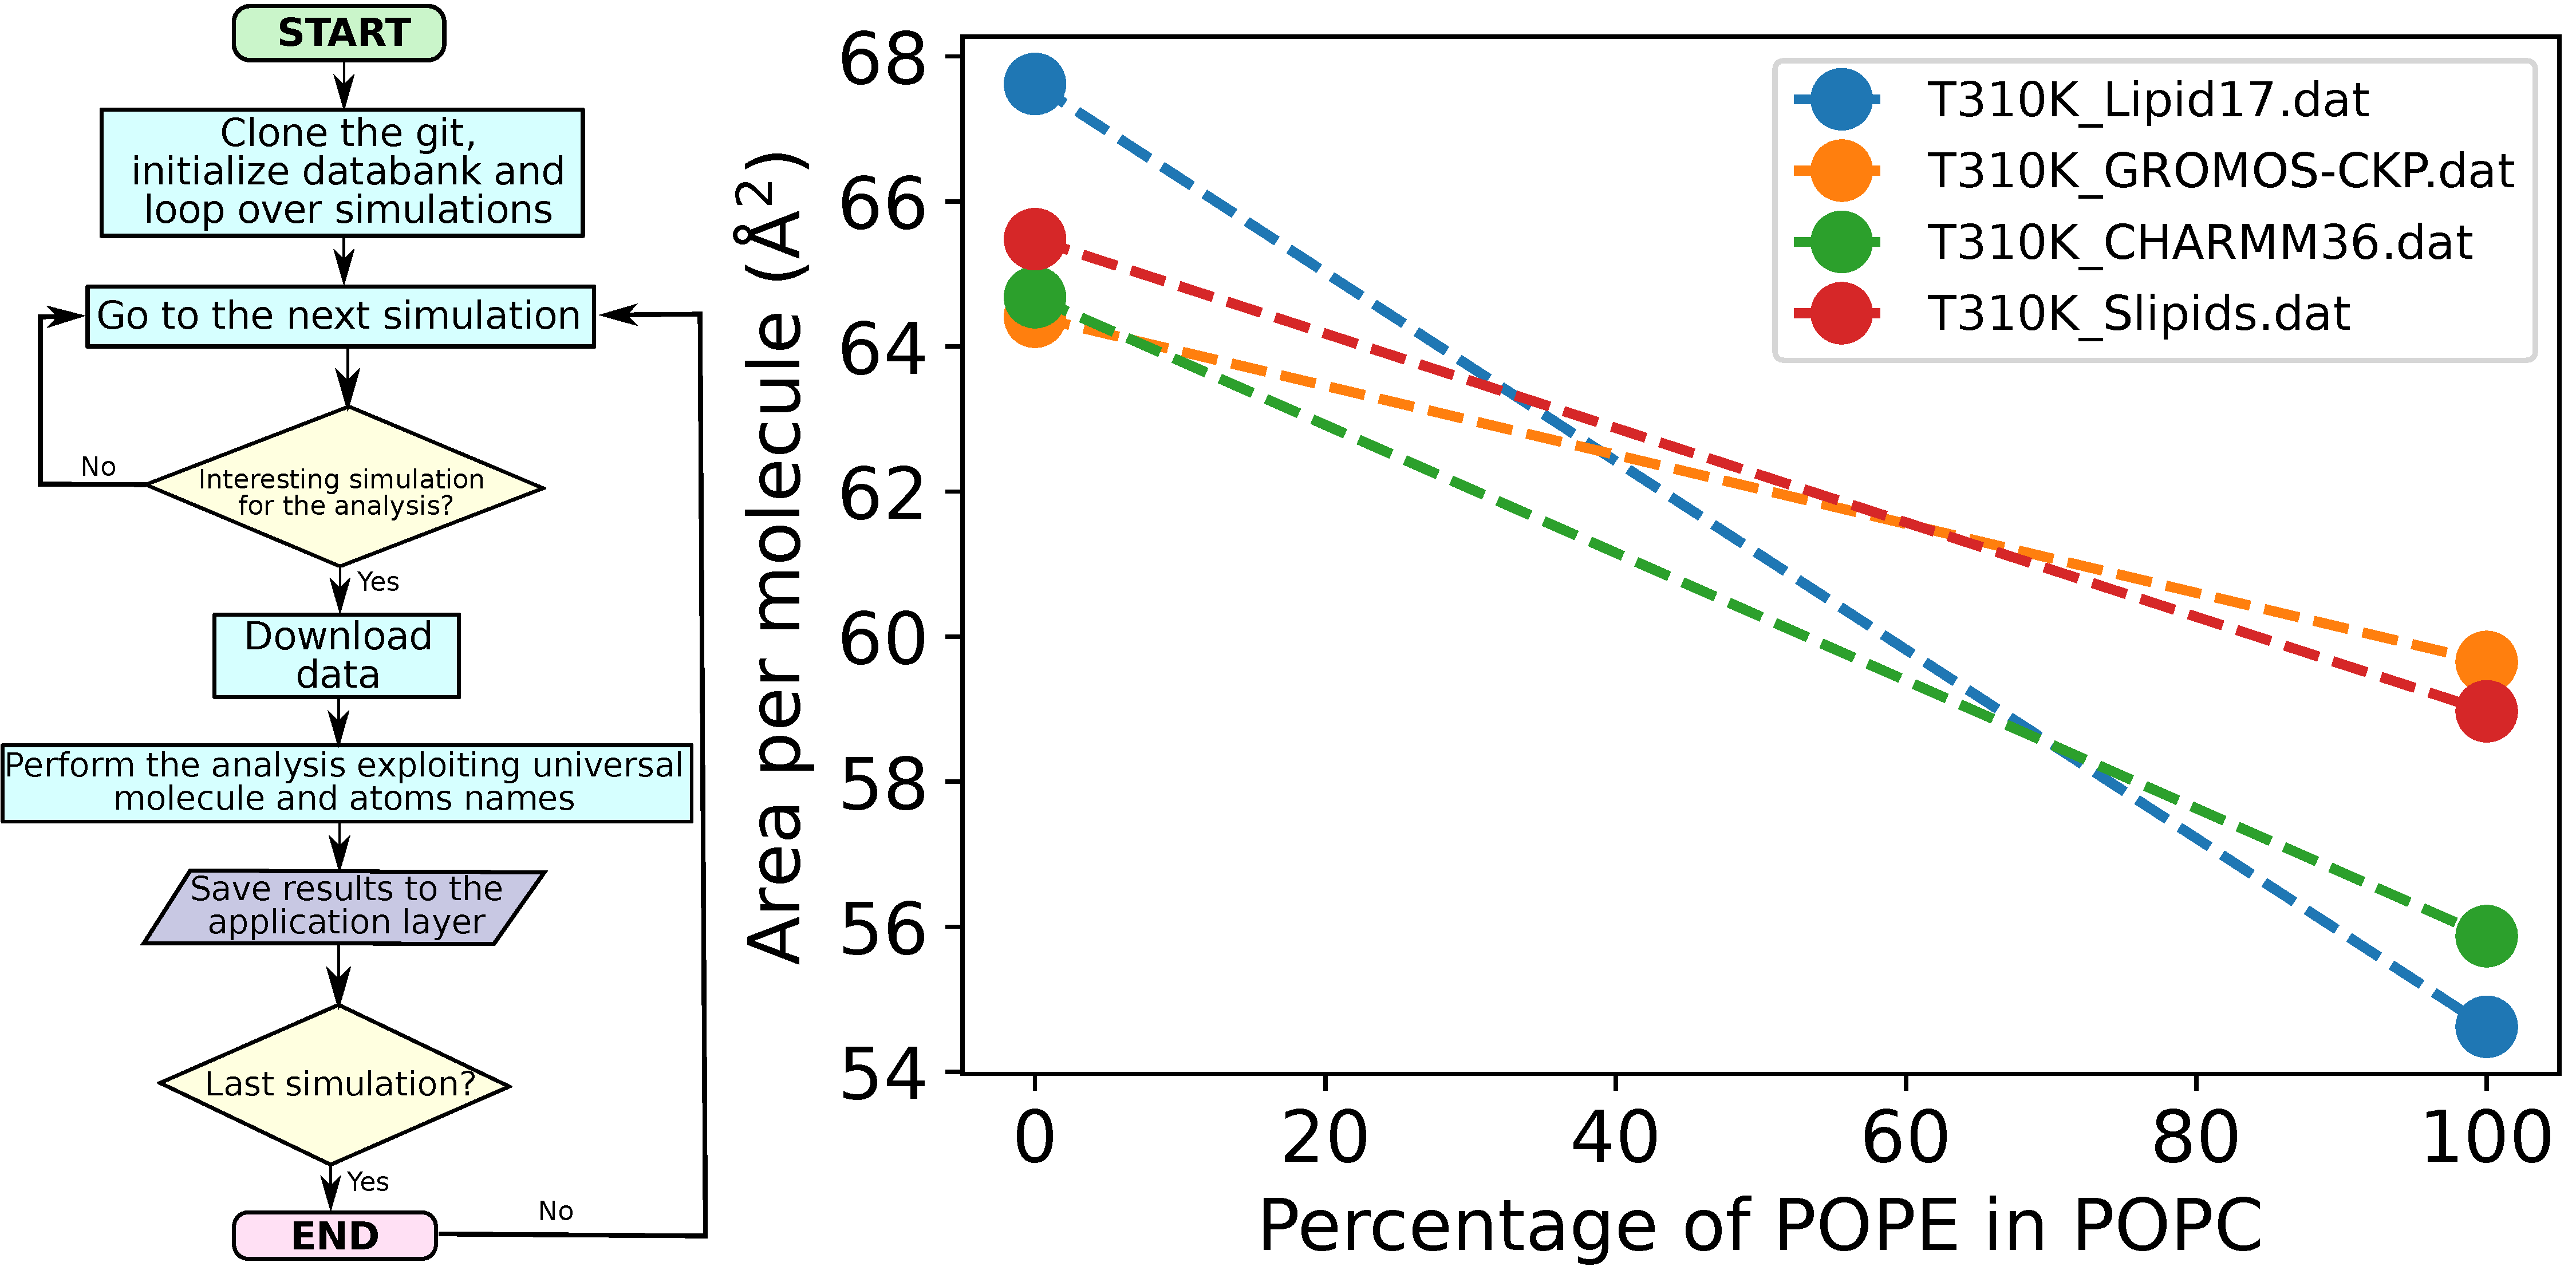
\includegraphics[width=88mm]{Figures/flowchart2.pdf}
    \caption{ A) Flowchart for performing an analysis of properties through all MD simulations in the NMRlipids databank using the API.
    B) Flowchart for accessing results calculated from the NMRlipids databank and stored to the application layer.
    C) Area per lipids of POPC and POPE lipid bilayers predicted by different force fields at 310\,K in simulations that are available in the NMRlipids databank. The points from the best performing simulations in the NMRlipids databank quality evaluation for each lipid (Figs.~\ref{fig:quality} and~\ref{fig:POPC_POPE_dataSI}) are surrounded by black circles. 
    }
    \label{fig:POPCPOPEapls}
\end{figure}

\subsection{Applications of the NMRlipids databank}
\subsubsection{Selection of simulation parameters using the NMRlipids databank: Best models for most abundant neutral membrane lipids}
%Quality of membrane simulations with different force fields have been evaluated against experimental data during parameterization and in separate comparison studies~\cite{botan15,ollila16,catte16,pluhackova16,perez17,leonard19,??}, but the lack of universal quality measure for membrane simulations complicates the estimations of reliability of simulations. 
Understanding of how closely simulations resemble the reality is crucial for selecting best models for specific applications, assessing the reliability and significance of MD simulation results, and using atomistic simulations in parametrization of coarse grained models. However, undefined universal quality measures for MD simulations and the lack of a prevailing force field that would perform best in all simulations has led to many controversial results in membrane simulations~\cite{antila22b}. 
%For example, OPLS3e parameters overcome CHARMM36 in structural quality for POPC but predicts overestimated ion binding~\cite{kurki22}. On the other hand, CHARMM36 gives the best description for lipid headgroup conformational ensembles~\cite{bacle21}, while GROMOS-CKP parameters best capture the membrane packing in POPS bilayers~\cite{antila22b}. 
For example, Fig.~\ref{fig:POPCPOPEapls}B illustrates divergent predictions from different force fields for the lateral packing of POPC and POPE membranes that are the two most biologically abundant neutral membrane lipids~\cite{vanmeer08}. We have previously resolved such controversies for membrane structures and ion binding affinities for neutral~\cite{botan15,catte16} and charged lipids~\cite{antila19,bacle21} by comparing simulations with C-H bond order parameters from NMR, yet this requires manual comparisons between large number of simulations. To streamline this process,
%the selection of best simulations for specific applications, and to guide the development of atomistic and coarse grained parameters,
we have defined quantitative quality measures, based on C--H bond order parameters from NMR and X-ray scattering form factors, for lipid bilayer simulations in the NMRlipids databank. 
%The quality for each simulation in the NMRlipids databank with the corresponding experimental data available is currently done using C--H bond order parameters from NMR experiments and form factors from X-ray scattering experiments. 
The C--H bond order parameters are sensitive to conformational ensembles of individual lipid molecules~\cite{ollila16}, while correlating well also with the membrane thickness and lateral packing as shown in Fig.~\ref{fig:quality}F. The X-ray scattering form factors are related to membrane dimensions \textit{via} the electron density profile. In particular, locations of minima in these form factors are correlated with the membrane lateral packing and thickness as shown in Figs.~\ref{fig:quality}F,~\ref{fig:QualityCorrelationsSI}, and~\ref{fig:sizedependence}. For quantitative quality measures, probabilities for each order parameter to locate within experimental error, and the distance of the first form factor minimum from the experimental value are calculated from a simulation.
%For detailed definitions of quality measures, see the supplementary information.
Together with the API, these enable rapid and automatic quality evaluation of simulations in the NMRlipids databank, thereby promoting the selection of best simulations for specific applications without laborious force field evaluation, and automatic parametrization procedures for atomistic and coarse grained simulations.

To select the best models for POPC and POPE among simulations compared in Fig.~\ref{fig:POPCPOPEapls}C, we show the ranking based on C--H bond order parameter quality in Fig.~\ref{fig:quality}A for the best performing simulations in the NMRlipids databank, and for the best performing POPE lipid bilayer simulations in Fig.~\ref{fig:quality}B. Direct comparisons with experiments are shown for selected simulations in Figs.~\ref{fig:quality}C--E and~\ref{fig:POPC_POPE_dataSI}. 
%The power of the NMRlipids databank in selecting the best simulation parameters for a specific application is demonstrated for mixtures of PE and PC lipids in Fig.~\ref{fig:POPCPOPEapls} showing area per lipids from available POPC and POPE bilayer simulations in the databank from different force fields at 310\,K. Predictions from different force fields deviate significantly in terms of absolute values and the slope of decrease upon addition of POPE. 
Because the area per lipid correlates with the average order parameter of the $\textit{sn}$-1 chain (Fig.~\ref{fig:quality} F), quality evaluation in Fig.~\ref{fig:quality} and direct comparison in Fig.~\ref{fig:POPC_POPE_dataSI} can be used to select the simulations that best capture area per lipids for POPE and POPC lipids in Fig.~\ref{fig:POPCPOPEapls}C. In these results, simulations with Slipids parameters ranks 1\textsuperscript{st} for POPC with a clear difference to others, and 2\textsuperscript{nd} for POPE with only marginally lower quality than GROMOS-CKP. Simulations with CHARMM36 and GROMOS-CKP parameters predict overly packed bilayer for POPC (overestimated order in Fig.~\ref{fig:POPC_POPE_dataSI}), while the area per lipid for POPC is overestimated in Lipid17. For POPE, CHARMM36 and Lipid17 predict membranes that are too packed. In conclusion, the quality evalution based on the NMRlipids databank suggests that Slipids parameters are the best available choice for simulations with PC and PE lipids, at least for the cases were membrane packing is relevant.

\begin{figure}[!t]
    \centering
    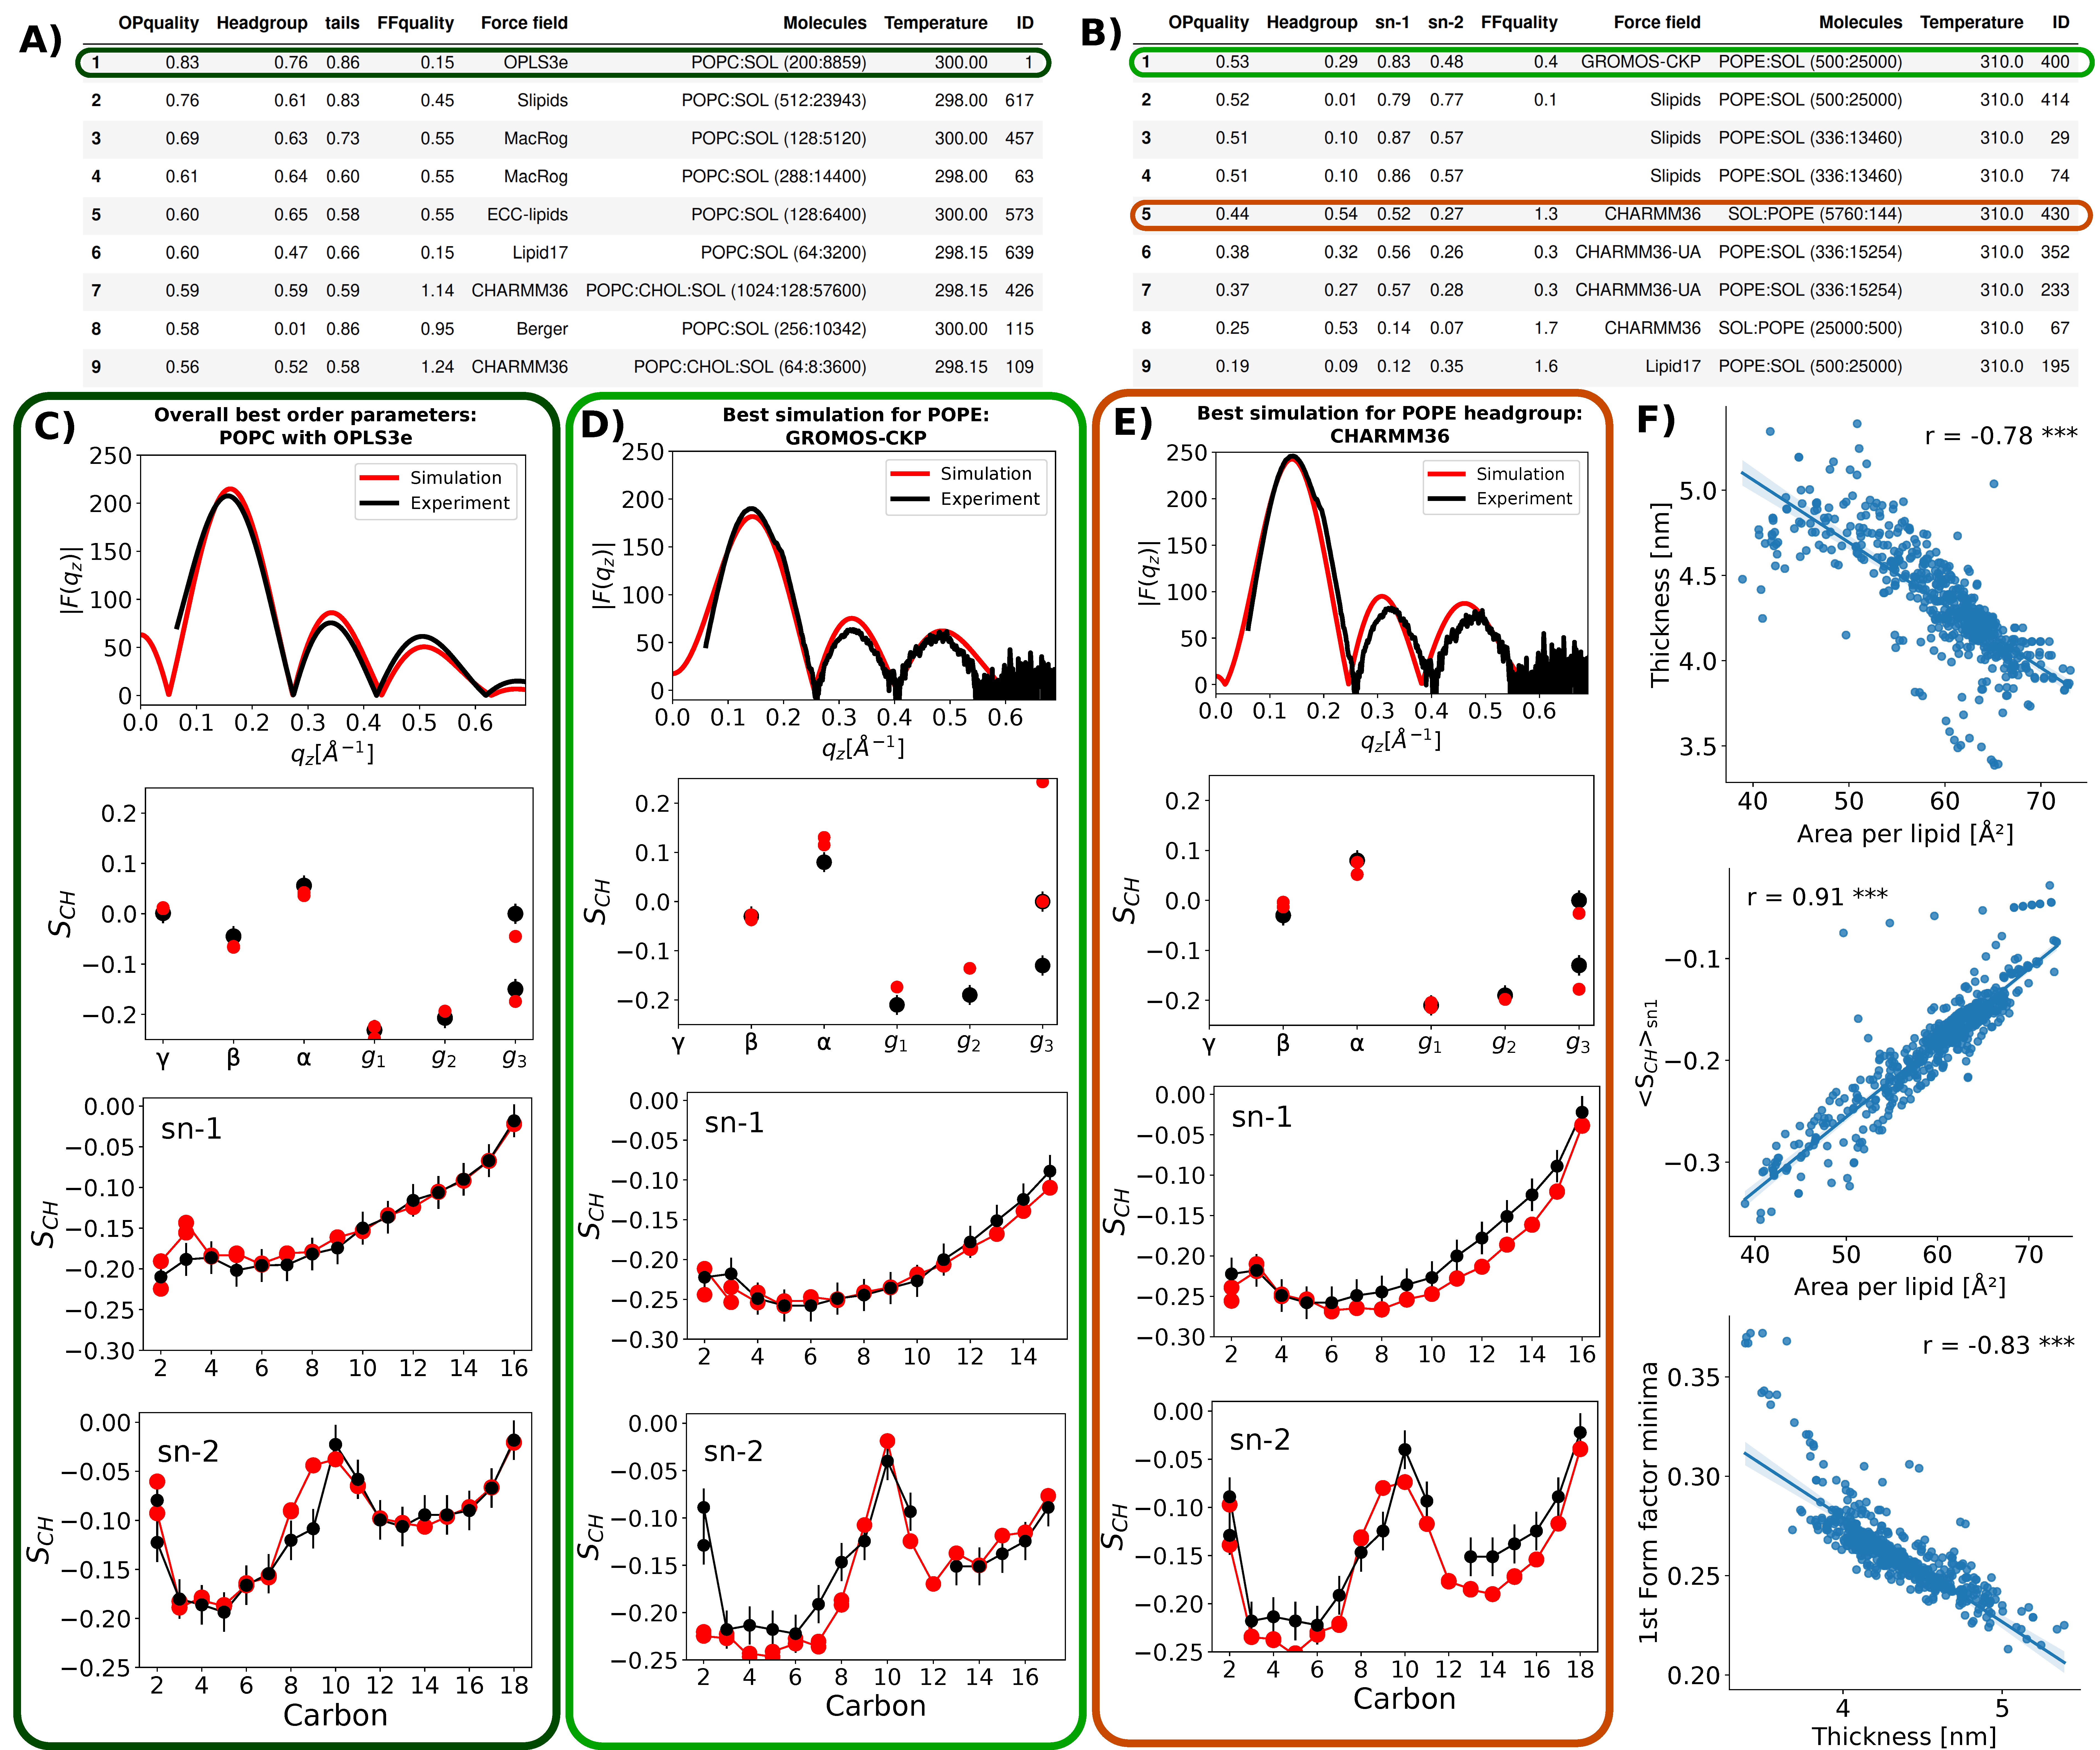
\includegraphics[width=\linewidth]{Figures/quality3.pdf}
    \caption{ A) Best simulations ranked based on overall order parameter quality.
    B) Best simulations ranked based on the overall order parameter quality of POPE lipid. 
    C)--E) Evaluation against experimental (NMR order parameters and X-ray scattering ) data exemplified for a simulation with the best overall order parameter quality (C), the best quality for POPE lipid (D), and the headgroup quality for POPE (E).
    F) Scatter plots and Pearson correlation coefficients, $r$, for the membrane area per lipid, thickness, first minimum of X-ray scattering form factor and average order parameter of the {\textit sn}-1 acyl chain extracted from the NMRlipids databank. All correlation coefficients have p-value below 0.001 as indicated by $^{***}$. For more correlations see Fig.~\ref{fig:QualityCorrelationsSI}.
    }
    \label{fig:quality}
\end{figure}


%In summary, the automatic quality evaluation of the NMRlipids databank enables the rapid exploration and selection of the best simulation parameters for specific applications without extensive and tedious manual force field evaluation. This possibility will promote more reliable simulation results for wide range of applications, support force field development, and streamline the parametrization of coarse grained force fields against the best atomistic MD simulations. The automatically extracted quantitative quality measures will be particularly useful to guide automatic parametrization procedures.

%Understanding such complex picture of lipid bilayer MD simulation quality would not be possible without automatic quality evaluation of large sets of simulations enabled by the NMRlipids databank.






\subsubsection{Detecting rare phenomena using NMRlipids databank: Cholesterol flip--flops}
Lipid flip--flops from one bilayer leaflet to another play an important role in lipid trafficking and regulating membrane properties~\cite{vanmeer08}. Phospholipid flip--flops are slow when not facilitated by proteins, occurring spontaneously on the timescale of hours or days, while cholesterol, diacylglycerol and ceramide flip-flops are faster. Still, the reported timescales range from minutes to sub-millisecods~\cite{vanmeer08,steck12,parisio16,gu19}. These timescales were previously accessible only by coarse-grained simulations or free energy calculations~\cite{parisio16}, yet atomistic simulations reporting cholesterol flip--flop events have been published only recently~\cite{gu19,javanainen19,baral20}. These studies report an increase in cholesterol flip--flop rates with increasing acyl chain unsaturation level and decreasing cholesterol concentration~\cite{gu19,javanainen19}, but the amount of data in these individual studies was not sufficient to systematically assess correlations between cholesterol flip--flop rates and membrane properties. Here, we demonstrate that the NMRlipids databank API makes analyses of such rare phenomena accessible to everyone by enabling the access to large amount of MD simulation data as described in section~\ref{section:access}. This is particularly useful for scientists in different fields of science and industry who do not have the access to required computational resources and expertise to produce the large amounts of MD simulation data. 


Using workflow depicted in Fig.~\ref{fig:POPCPOPEapls}A, we first calculated the cholesterol flip--flop rates from all the simulations available in the NMRlipids databank. Flip--flops were observed for cholesterol, % (634 events in 77 different simulations), 
DCHOL (18,19-di-nor-cholesterol), %, 16 flip-flops in 1 simulation) 
DOG (1,2-dioleoyl-\textit{sn}-glycerol), %, 44 flip-flops in 4 simulations) 
and SDG (1-stearoyl-2-docosahexaenoyl-\textit{sn}-glycerol). The observed cholesterol flip--flop rates, ranging between 0.001--1.6\,\textmu{}s$^{-1}$ with the mean of 0.16\,\textmu{}s$^{-1}$ and median of 0.07\,\textmu{}s$^{-1}$, are in line with the previously reported values from atomistic MD simulations~\cite{gu19,javanainen19,baral20}. The flip--flop rate of DCHOL, 0.2\,\textmu{}s$^{-1}$, was close to the average value of cholesterol, while average rates for diacylglycerols DOG and SDG were higher than for cholesterol, 0.4\,\textmu{}s$^{-1}$ and 0.5\,\textmu{}s$^{-1}$, respectively. Flip--flops were not observed for other lipids, giving the upper limits for PC lipid flip--flop rate of 9$\cdot$10$^{-6}$\,\textmu{}s$^{-1}$ and for ceramide (\textit{N}-palmitoyl-\textsc{D}-\textit{erythro}-sphingosine) of 0.002\,\textmu{}s$^{-1}$. Thus, available data in the NMRlipids databank suggests that the lipid flip--flip rate decreases in the order of diacylglycerols $>$ cholesterol $>$ other lipids including ceramides. However, the amount of data for diacylgycerols (8 simulations with Lipid17 force field) and ceramide (3 simulations with CHARMM36 force field) is less than for cholesterol (83 simulations), thus we cannot fully exclude the effect of force field or composition on this comparison.

Nevertheless, we used the workflow depicted in Fig.~\ref{fig:POPCPOPEapls}B to analyse how flip--flop rates calculated from the NMRlipids databank depend on membrane properties. Cholesterol flip--flop rates and their histograms are plotted as a function of membrane thickness, lateral density and order in Figs.~\ref{fig:flip-flops} B--D. The results reveal a non-linear correlation between cholesterol flip--flop rate and membrane packing which is depicted as area per lipid. Flip--flop rates increase by an order of magnitude when membrane packing density decreases and a major jump is observed at low membrane packing. The order of magnitude changes in cholesterol flip--flop rate with the membrane composition may have major implications in understanding lipid trafficking and membrane biochemistry~\cite{gu19,baral20}. Because the results from the NMRlipids databank are averaged over large range of membrane compositions and force fields, they show that the strong dependence of cholesterol flip--flop rate on membrane properties is not limited to certain lipid compositions or force fields used in previous studies~\cite{gu19,javanainen19,baral20}.

\begin{figure}[htb]
    \centering
    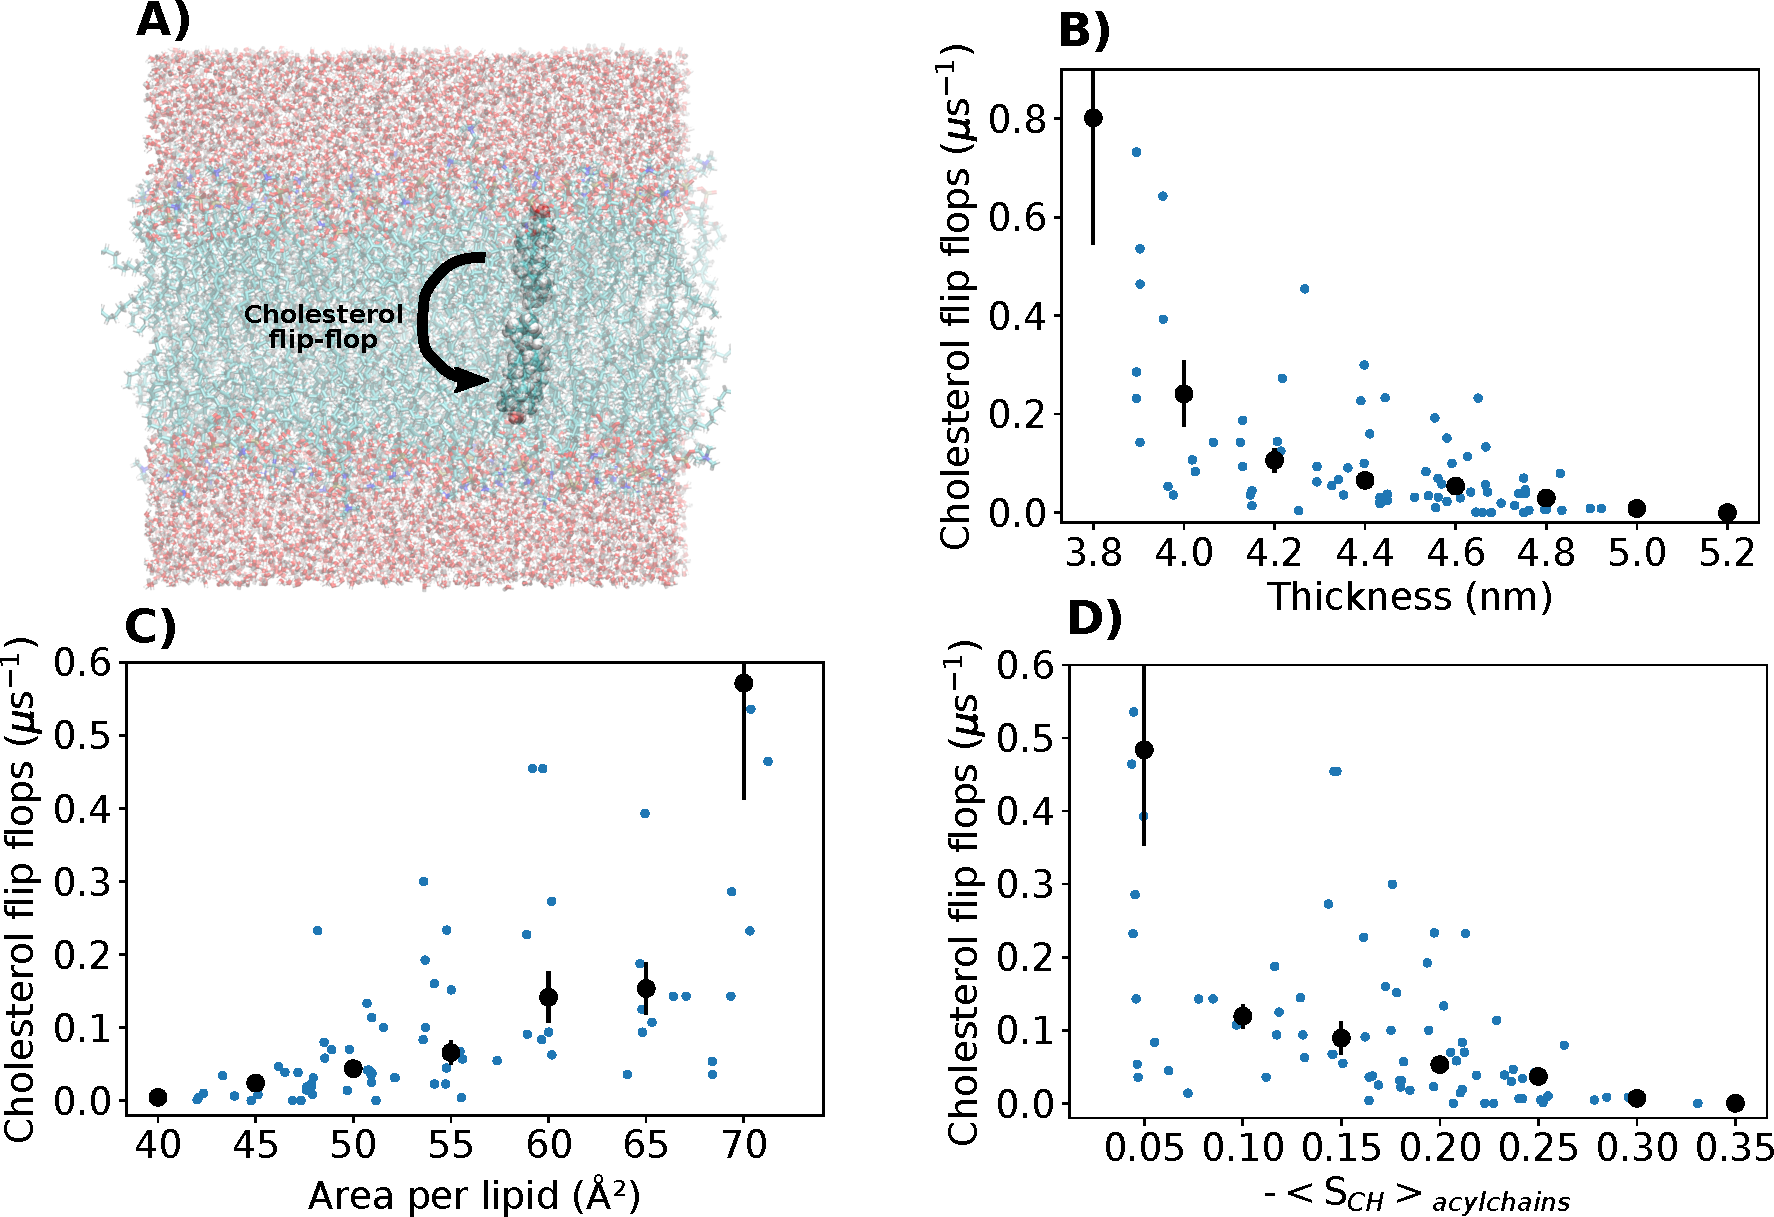
\includegraphics[width=88mm]{Figures/CholFlipFlops.pdf}
    \caption{\textbf{A} Illustration of cholesterol flip--flop.  
      \textbf{B--D} Cholesterol flip--flops analyzed from the databank as a function of membrane thickness, area per lipid, and acyl chain order. Values from simulations with non-zero flip--flop rates are shown with blue dots. Histogrammed values are shown with black dots.
    }
    \label{fig:flip-flops}
\end{figure}



\subsubsection{Extending the scope of MD simulations to new fields using the NMRlipids databank: Water diffusion anisotropy in membrane systems}
The anisotropy in water diffusion in parallel and perpendicular directions with respect to membranes can be related to the translocation of drugs  through biological material, particularly in skin \cite{hansen13,wen18,nitsche19,roberts21}, and to the formation of signals in diffusion tensor MRI imaging~\cite{topgaard20}. MD simulations are rarely used to analyze the anisotropic diffusion of water since only few membrane permeation events for water are typically observed in a single MD simulation trajectory~\cite{venable19,camilo2022}, thereby making the collection of sufficient amount of data challenging. Here, we show that the API access to the data in NMRlipids databank enables systematic analyses on how the anisotropic diffusion of water depends on membrane properties in multilamellar membrane systems, thereby extending the applications of MD simulations to new fields. 

\begin{figure}[tb]
    \centering
    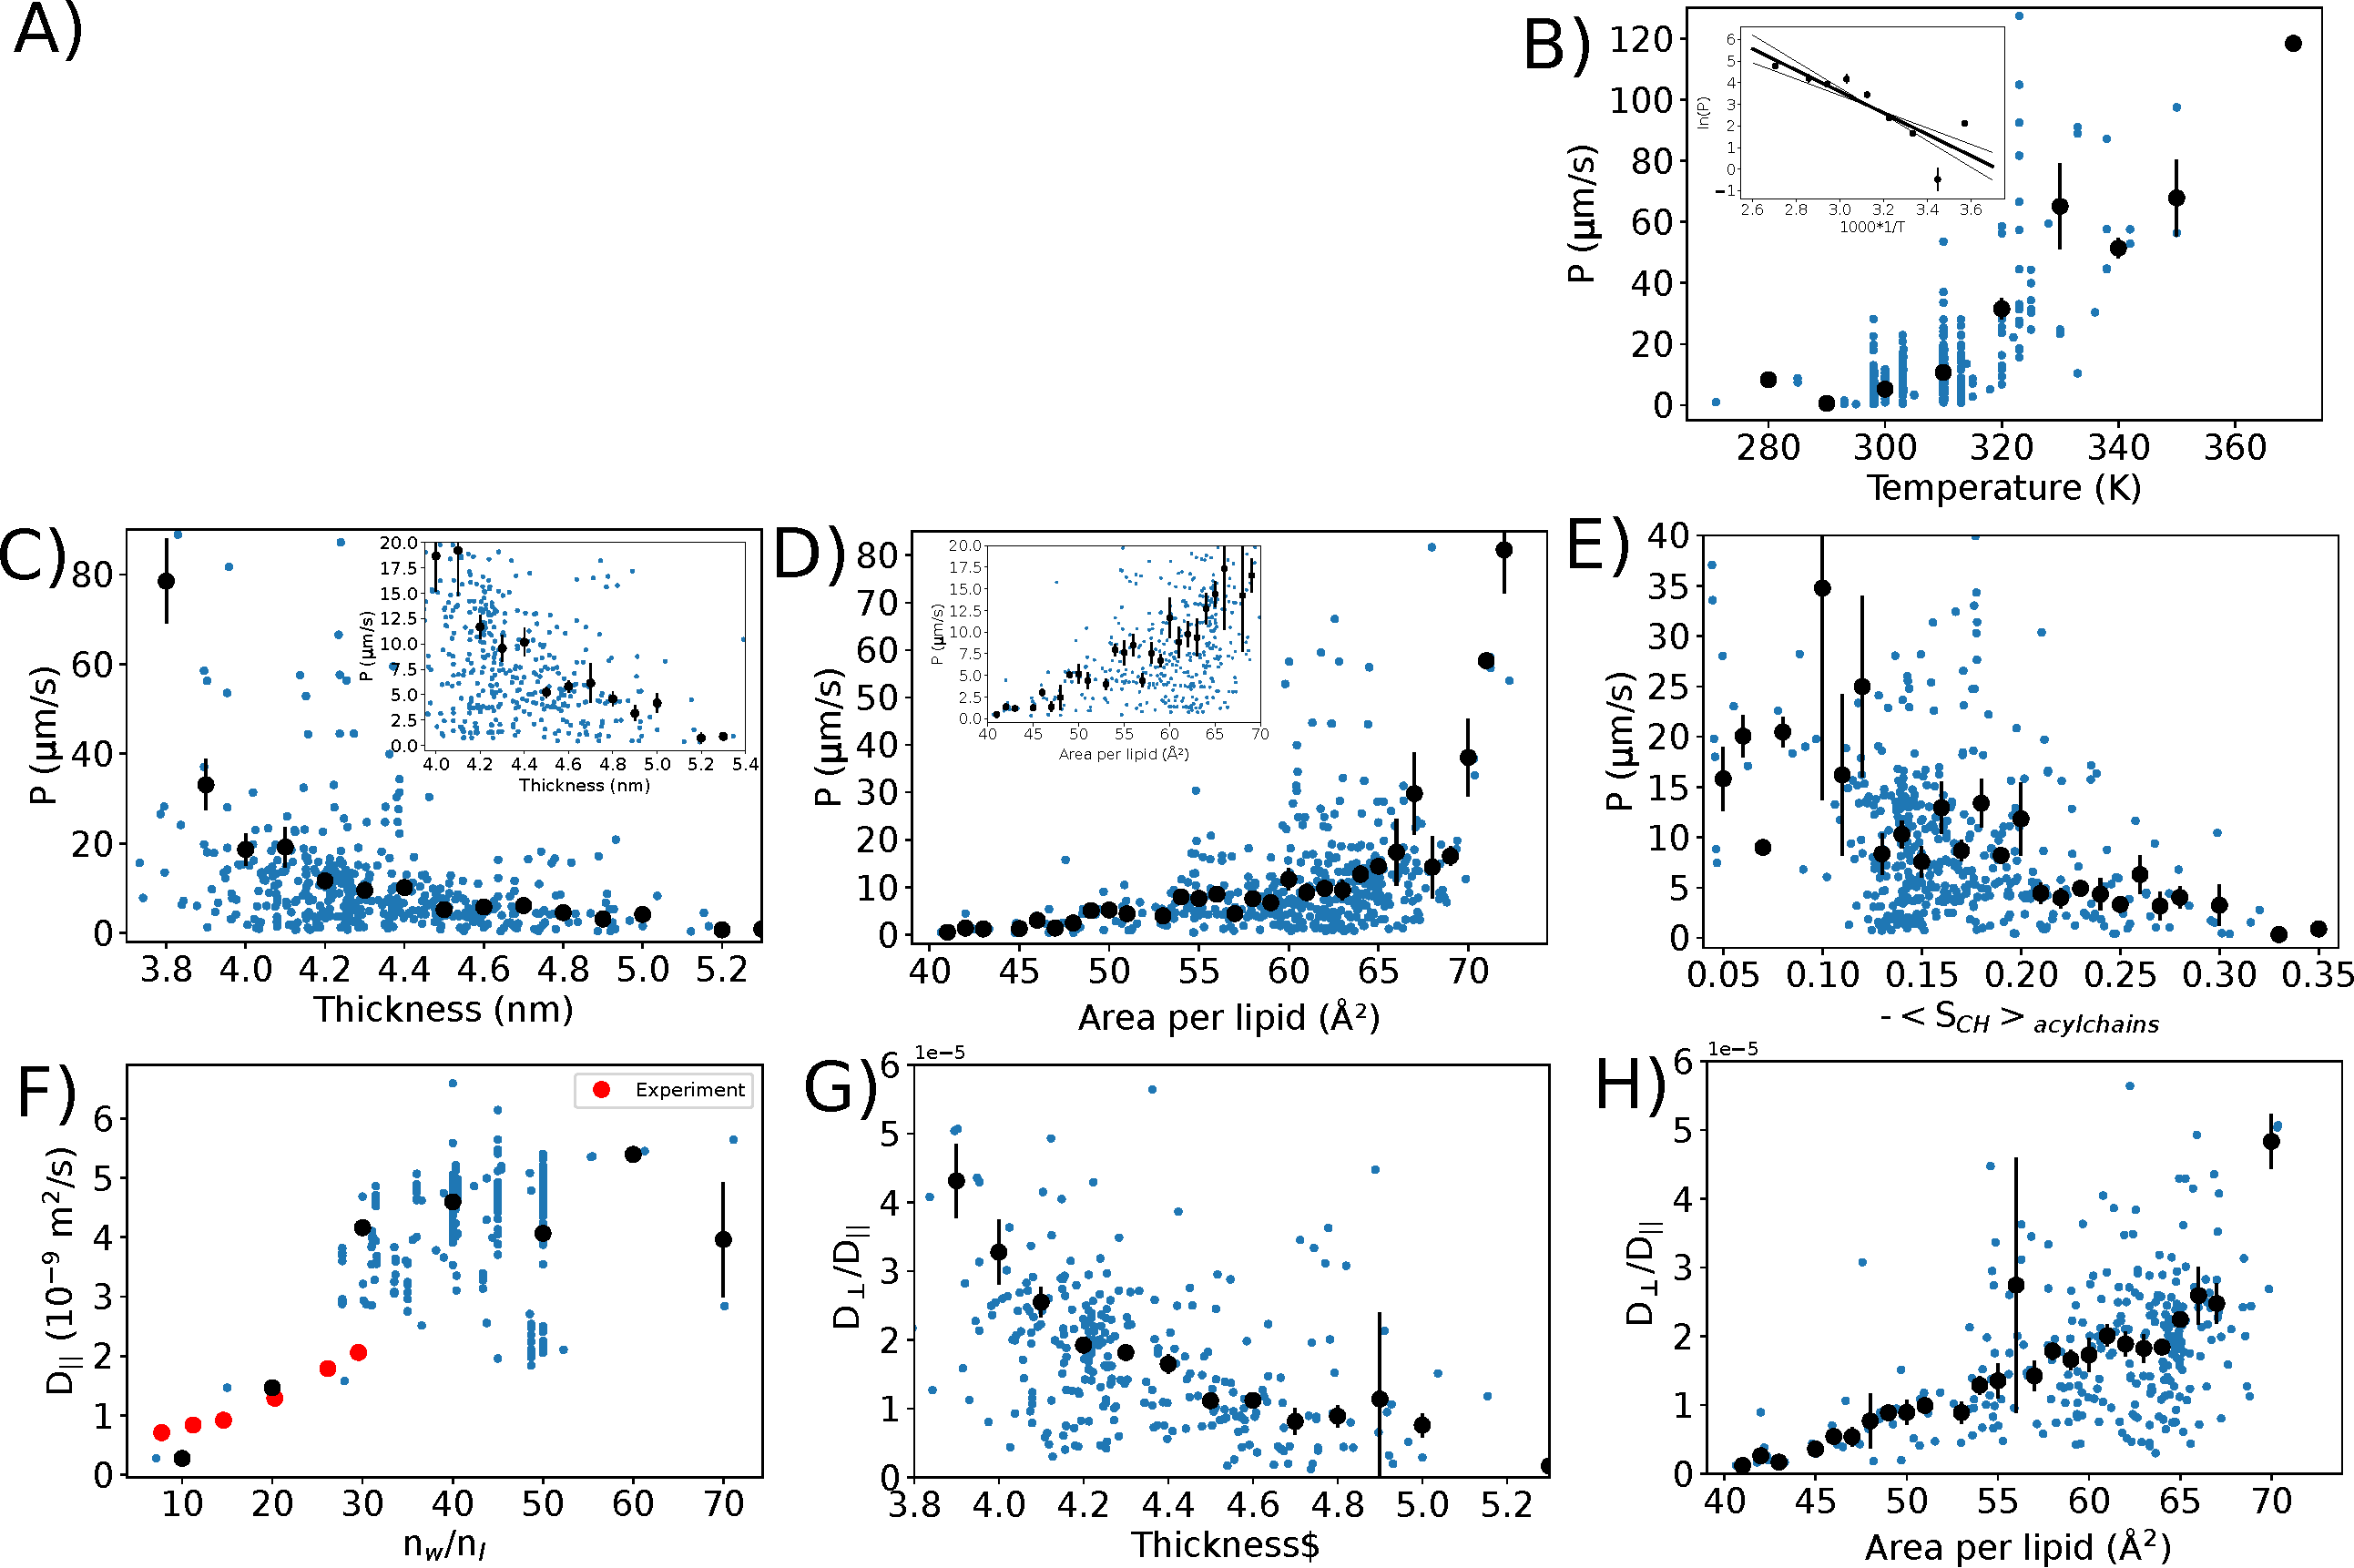
\includegraphics[width=\linewidth]{Figures/permeation2.pdf}
    \caption{\textbf{A} Water diffusion, $D_\mathrm{perp}$, and permeability, $P$, through membranes, and lateral diffusion along the membrane, $D_{||}$, illustrated in a multilamellar stack of lipid bilayers. 
    \textbf{B--E} Water permeation through membranes analyzed from the databank as a function of temperature, thickness, area per lipid, and acyl chain order. Values from simulations with non-zero permeation values are shown with blue dots. Histogrammed values are shown with black dots. Inset in B) shows the Arrhenius plot of permeation ($\ln(P)$ vs. $1/T$) that gives 17\,$\pm$\,4\,$k_\mathrm{B}T$ for the average activation energy for water permeation through lipid bilayer. Insets in C) and D) show the region where the dependence could be considered approximately linear.
    \textbf{F} Lateral diffusion of water as a function of hydration level. Experimental points for DMPC bilayers at 313\,K at different hydration levels are shown~\cite{rudakova04}.
    \textbf{G--H} Diffusion anistoropy of water as a function of thickness and area per lipid. }
    \label{fig:permeability}
\end{figure}


To this end, we first calculated the water permeability through membranes from all simulations in the NMRlipids databank using the workflow depicted in Fig.~\ref{fig:POPCPOPEapls}A. The resulting non-zero values range between 0.3 and 322\,\textmu{}m/s with the mean and median of 14\,\textmu{}m/s and 8\,\textmu{}m/s, respectively. These values agree with the previously reported simulation results~\cite{venable19,camilo2022}, but are on average slightly larger than experimental values reported for PC lipids in the liquid crystalline phase,~0.19--0.33\,\textmu{}m/s~\cite{jansen95}. Using the workflow depicted in Fig.~\ref{fig:POPCPOPEapls}B, we then plotted the observed permeabilities and their histogrammed values in Figs.~\ref{fig:permeability}B--E as a function of temperature, membrane thickness, area per lipid, and acyl chain order. As expected, the permeability increases with the temperature, giving an average energy barrier of 17\,$\pm$\,4\,$k_\mathrm{B}T$ for the water permeation from the Arrhenius plot in Fig.~\ref{fig:permeability}B. On the other hand, the permeability of water decreases on average when membranes become more packed, \textit{i.e.}, with decreasing area per lipid and increasing thickness and acyl chain order (Figs.~\ref{fig:permeability} C--E). Permeation of water through bilayers depends on membrane properties also according to previous studies, but there is no established consensus on whether the area per lipid~\cite{nagle08} or bilayer thickness~\cite{frallicciardi22} is the main parameter determining the permeability. 
%is previously reported from simulations and experiments for some systems, but not for all~\cite{mathai07,venable19,frallicciardi22}. 
Our analysis over the NMRlipids databank, containing significantly more data than what was available in previous studies, suggest non-linear dependencies on both of these parameters, yet the linear correlation would be a good approximation for thicknesses above $\sim$\,3.9\,nm and area per lipids below $\sim$69\,\AA{}$^2$ (insets in Figs.~\ref{fig:permeability} C--D).
%within the range of experimentally reported values  permeability which is 1-2 orders of magnitude slower than osmotic permeability \cite{jansen95,??}. 
Clear dependencies of permeability on charged lipids, cholesterol, POPE, or hydration level were not observed in Fig.~\ref{fig:permeationSI} in the supplementary information.
%, although weak decrease for the latter two may be visible.
%
%
%
%%Several models on how water dynamics depends on membrane properties have been proposed based on different experimental and %%theoretical methods, yet consensus 
%%%on how water permeability depends on membrane properties, such as area per lipid and thickness, or molecular composition, 
%%has not been reached~\cite{mathai07,nitsche13,nitsche16,shinoda16,venable19,frallicciardi22}.  


To analyze how water diffusion anisotropy depends on membrane properties in a multi-lamellar lipid bilayer system, we calculated the water diffusion parallel to the membrane surface from all simulations in the NMRlipids databank using the workflow depicted in Fig.~\ref{fig:POPCPOPEapls}A. The parallel diffusion coefficient of water, $D_{||}$, decreases with reduced hydration and increases with the temperature, but dependencies on membrane area per lipid, thickness, or fraction of charged lipids were not observed in Figs.~\ref{fig:permeability} and~\ref{fig:diffusionSI} when the workflow depicted in Fig.~\ref{fig:POPCPOPEapls}B was used. Simulation results are close to the experimental values with low hydration levels in Fig.~\ref{fig:permeability} F, but increase to approximately two times higher than the experimental value for bulk water diffusion value (3.1$\cdot$\,10$^{-9}$\,m$^2$/s at 313\,K~\cite{khakimov08}) with high hydration levels. This is not surprising as the most common water model used in membrane simulations, TIP3P, overestimates the bulk water diffusion~\cite{pathirannahalage21}. To estimate the diffusion anisotropy of water, $D_\mathrm{\perp}/D_{||}$, in multilamellar membrane system, the permeability coefficients of water through membranes were translated to perpendicular diffusion coefficients, $D_\mathrm{\perp}$, using the Tanner equation~\cite{tanner78,wasterby02}. The resulting perpendicular diffusion coefficients are approximately five orders of magnitude smaller than lateral diffusion coefficients of water (Figs.~\ref{fig:permeability} G and H), which is at the upper limit of the anisotropy estimated from the experimental data~\cite{nitsche19}. 
%Large anisotropy values are understandable as simulations give slightly slower permeation rates and higher lateral diffusion rates than experiments. 
Significant increase in the diffusion anisotropy with membrane packing is observed, as $D_\mathrm{\perp}/D_{||}$ drifts away from one with decreasing area per lipid and increasing thickness in Figs.~\ref{fig:permeability} G and H. This follows from decreasing water permeability with membrane packing (Figs.~\ref{fig:permeability} C and D), while lateral diffusion remains approximately constant (Figs.~\ref{fig:diffusionSI} A and C). 

In summary, our results suggest that the bilayer packing has a substantial effect on anisotropic water diffusion in multi-membrane lipid systems. Several folds larger anisotropy in membranes with higher lateral density is expected to play a role in pharmacokinetic models not only for water but also for other hydrophilic molecules~\cite{nitsche19}. Furthermore, the enhanced understanding of this anisotropy may help in developing new diffusion tensor based MRI imaging methods where signals originate from anisotropic diffusion of water in biological material~\cite{topgaard20}.

\section{Discussion}

%The Discussion should be succinct and must not contain subheadings.

The focus of biomolecular simulations is moving from studies of individual molecules to larger complexes and even whole cells and organelles~\cite{johnson15,thornburg22,gupta22}. Simultaneously, machine learning based models predicting behaviour of biomolecules and automatic approaches to parametrize models are emerging~\cite{jumper21,antila22b}. The NMRlipids databank will support the development in both of these directions. The automatic quality evaluation and ranking of simulations in the NMRlipids databank guides the optimization of new force field parameters and the selection of best parameters for large biomolecular complexes where simulation quality becomes increasingly important due the accumulation of small errors in large simulations. Furthermore, the NMRlipids databank serves as a training set for diverse machine learning applications. For example, a machine learning model predicting electron density profiles from form factors would be highly useful in interpretation of scattering experiments. In addition, the data contained in the NMRlipids databank will enable training of more elaborated models to predict arbitrary membrane properties. 


%The NMRlipids databank will be of great benefit to scientists involved in MD simulations. They will be able to rapidly evaluate the quality of MD simulations in order to filter out potentially misleading results or facilitate force field parameter development~\cite{antila22b}. The selection of best models for a specific application is demonstrated for PC/PE lipid mixtures in Fig.~\ref{fig:quality}, and previously for PC/PS lipid mixtures~\cite{antila22b}, and lipid headgroups~\cite{bacle21}. 
The programmatic access in the NMRlipids databank enables automatic analyses of structural and dynamic properties over larger sets of simulation data in terms of quantity (\textit{e.g.}, simulation length and number of conformations) and content (\textit{e.g.}, lipid compositions and ion concentrations) than is currently possible by a single research group. The added value of such analyses is demonstrated here by analysing the anisotropic diffusion of water in membrane systems (Fig.~\ref{fig:permeability}) and cholesterol flip--flop events (Fig.~\ref{fig:flip-flops}). By enabling these analyses for everyone, the NMRlipids databank can lead to applications in unprecedented directions in fields where MD simulations are less commonly utilized, such as pharmacokinetic modeling and in MRI imaging where anisotropic diffusion of water play important roles~\cite{nitsche19,topgaard20}. 
Different types of applications enabled by the NMRlipids databank across a wide range of fields are exemplified in Table~\ref{tab:applications}. The ever growing amount of data is expected to further increase the scope of potential applications of the NMRlipids databank in biology, biotechnology, material science, biomolecular imaging and beyond. 

\begin{table}[t]
    \centering
    \begin{tabular}{p{5.0cm}  p{5.0cm}  p{4.0cm}}
    Type of application     & Practical examples & Target group \\
    \hline
    Analyses of rare phenomena               & Lipid flip--flops, water permeation (Figs.~\ref{fig:flip-flops} and~\ref{fig:permeability}) & Membrane scientists \\
    \\
    Correlations between membrane properties & 
    Membrane structural properties, water dynamics (Figs.~\ref{fig:quality} and~\ref{fig:permeability}) & 
    Membrane scientists \\
    \\
    Applications that are outside typical scope of MD simulations & 
    Anisotropic water diffusion for pharmacokinetics and MRI imaging applications (Fig.~\ref{fig:permeability}) & 
    Scientist in fields where MD simulations are not usually applied \\
    \\
    Selection of the best simulation model for a specific application & 
    Best model for POPC lipids (Fig.~\ref{fig:quality}), headgroup conformations~\cite{bacle21}, 
    packing of PS~\cite{antila22b} and PE (Fig.~\ref{fig:POPCPOPEapls}) containing membranes. &
    Scientists using MD simulations \\
    \\
    Guidance for force field development & 
    Improvements in ion binding to lipids~\cite{melcr18,melcr20} and lipid headgroup conformational ensembles~\cite{yu21,dickson22,grote20} &
    Scientists developing parameters for MD simulations \\
    \\
    Training and target data for coarse grained models & 
    Optimizing parameters of coarse grained models against NMRlipids databank, extracting continuum parameters for membranes. &
    Scientists developing and using coarse grained MD simulations \\
    \\
    Training set for machine learning applicatons &
    Programmatic access to the data and results enables training of machine learning type of models for various applications, such as predictions of membrane properties from composition & Scientists building and using machine learning applications for biomolecules.  
    \end{tabular}
    \caption{Examples on applications of the NMRlipids databank.}
    \label{tab:applications}
\end{table}



The main practical limitations in building open access databanks of molecular dynamics simulations have been the required commitment in long term support for hardware and software maintenance, and the lack of incentives for researchers to share the data. The NMRlipids databank circumvents these challenges with the overlay databank design and open collaboration approach developed in the NMRlipids project~\cite{botan15}. In this model, the file storage is distributed to publicly available stable repositories (\textit{Data layer} in Fig.~\ref{fig:overlay} A) and maintenance of the databank does not depend on individual scientists or groups because all its version controlled content is available with an open access licence (\textit{Databank layer} in Fig.~\ref{fig:overlay} A). Incentive to share the data is created in the NMRlipids open collaboration by offering authorship in published articles to the contributors following the NMRlipids project protocol~\cite{botan15}. The current NMRlipids databank contains only lipid bilayer simulations, but the concept can also be applied to other biomolecules, such as disordered proteins and membrane-protein systems, or other fields where similar barriers to establish publicly accessible databanks exist. 



\newpage


\section{Methods}

%Topical subheadings are allowed. Authors must ensure that their Methods section includes adequate experimental and characterization data necessary for others in the field to reproduce their work.

\subsection{Structure of the databank}
Structure of the NMRlipids databank is illustrated more detailed in Fig.~\ref{DatabankStructure} in the supplementary information. The core content of the databank (\textit{Databank layer} in Fig.~\ref{fig:overlay}) locates as a git repository at \url{https://github.com/NMRLipids/Databank/} and is permanently stored in Zenodo repository (\url{www.zenodo.org})~\cite{??}. Whenever a specific file is referred here, the file path within the NMRlipids databank repository is given. The scripts in the NMRlipids databank are mainly written in Python and many of them utilize the MDAnalysis module~\cite{gowers2019mdanalysis,michaud2011mdanalysis}.

Essential information of each simulation in the NMRlipids databank is stored in a human and machine readable README.yaml file located at \texttt{/Data/Simulations} in the NMRlipids databank repository. These files contain access to all information that are needed for further analyses of simulations. The content of these files is described in detail in Table~\ref{tab:READMEkeys} in the supplementary information. Raw MD simulation data are stored in external publicly available and stable repositories (\textit{Data layer} in Fig.~\ref{fig:overlay}), such as Zenodo (\url{www.zenodo.org}), from where it can be downloaded whenever needed using the links in README.yaml files.  


\subsection{Molecule and atom naming convention} \label{naming}
When analysing simulations, atoms and molecules needs to be often called by their names defined in the simulation trajectory. However, these names typically vary between force fields because the universal naming convention has not been defined for lipids. To enable automatic analyses over simulations with different atom and molecule names in the NMRlipids databank, we have defined unique naming conventions for molecules and atoms therein. Unique abbreviations used in the NMRlipids databank for each molecule are listed in table~\ref{tab:abbreviations} in the supplementary information. Atom names used in simulation trajectories are connected to unique atom names using mapping files that are defined in the NMRlipids project (\url{https://nmrlipids.blogspot.com/2022/04/new-yaml-format-of-mapping-files.html}). These files are located at \texttt{/Scripts/BuildDatabank/mapping\_files} in the NMRlipids databank repository. These files also define whether an atom belongs to headgroup, glycerol backbone, or acyl chain region in a lipid. In practise, force field specific molecule names and mapping files
names are given in the COMPOSITION dictionary in README.yaml files for each molecule in each simulation in the NMRlipids databank.

\subsection{Adding data into the NMRlipids databank}
The NMRlipids databank is open for additions of simulation data by anyone. The first step is to create an info.yaml file containing the information that needs to be manually entered as listed in Table~\ref{tab:READMEkeys}. This file can be then added into \texttt{/Scripts/BuildDatabank/info\_files} folder in the NMRlipids databank repository via pull requests. After the pull request is manually accepted, the rest of the information for the README.yaml file, listed in Table~\ref{tab:READMEkeys}, will be automatically extracted using the \texttt{/Scripts/BuildDatabank/AddData.py} script. Currently, the NMRlipids databank is composed of simulations found from Zenodo repository with an appropriate licence. Most, but not all, of these trajectories originate from previous NMRlipids projects~\cite{botan15,catte16,antila19,bacle21}.

\subsection{Experimental data}
Experimental data used in the quality evaluation, currently composed of C--H bond order parameters and X-ray scattering form factors, are stored in \texttt{/Data/experiments} in the NMRlipids databank repository. Similarly to simulations, each experimental data set has a README.yaml file containing all the relevant information about the experiment. The keys and their descriptions for the experimental data are given in Table~\ref{tab:READMEkeysEXP}. NMR data currently in the NMRlipids databank are taken from Refs.~\citenum{scherer87,ferreira13,antila19,melcr20,bacle21} and X-ray scattering data from Refs.~\citenum{Kucerka08a,kucerka11,pan12b,pan14,kucerka15}. In addition, some previously unpublished NMR and X-ray scattering data are used. These are measured with previously established methods as described in the supplementary information. 


\subsection{Calculation of C--H bond order parameters}
The C--H bond order parameters were calculated directly from the carbon and hydrogen positions using the definition
%The order parameters are defined as
\begin{equation}\label{OP}
S_{\rm CH}=\frac{1}{2}\left\langle 3\cos^2\theta -1 \right\rangle,
\end{equation}
where angular brackets denote the ensemble average, \textit{i.e.}, average over all sampled configurations of all lipids in a simulation, and $\theta$ is the angle between the C--H bond and the membrane normal. As in previous NMRlipids publications, the order parameters were first calculated separately for each lipid and the standard error of the mean over different lipids was used as the error estimate~\cite{botan15}. The script that calculates C--H bond order parameters from all simulations in the NMRlipids databank is available at \texttt{/Scripts/AnalyzeDatabank/calcOrderParameters.py} in the NMRlipids databank repository. The resulting order parameters are stored for all simulations in files named %\newline 
[\texttt{lipid\_name}]\texttt{OrderParameters.json} at folders in \texttt{/Data/Simulations} in the NMRlipids databank repository.

\subsection{Calculation of X-ray scattering form factors}
X-ray scattering form factors were calculated with the standard equation for symmetric lipid bilayers~\cite{ollila16}
\begin{equation}\label{FFsimpl}
F(q)=\int_{-D/2}^{D/2}\Delta \rho_e(z) \cos(zq_z) {\rm d}z,
\end{equation}
where $\Delta \rho_e(z)$ is the difference between total and solvent electron densities, and $D$ is the simulation box size in the $z$-direction (normal to the membrane). For the calculation of density profiles, atom coordinates were first centred around the centre of mass of lipid molecules for every time frame, and a histogram of these centred positions, weighted with the number of electrons in each atom, was then calculated with the bin width of $1/3$~\AA{}. Electron density profiles were then calculated as an average of these histograms over the time frames in simulations. The script to calculate form factors for all simulations in the NMRlipids databank is available at \texttt{Scripts/AnalyzeDatabank/calc\_FormFactors.py}. The resulting form factors are stored for all simulations in files named \texttt{FormFactor.json} at folders in \texttt{/Data/Simulations} in the NMRlipids databank repository.

\subsection{Calculation of a bilayer area per lipid and thickness}
Area per lipids of bilayers were calculated by dividing the time-averaged area of the simulation box with the total number of lipid and surfactant molecules (see the list in table~\ref{tab:abbreviations}) in the simulation. The script that calculates area per lipids from all simulations in the NMRlipids databank repository is available at \texttt{Scripts/AnalyzeDatabank/calcAPL.py} in the NMRlipids databank repository. The resulting area per lipids are stored for all simulations in files named \texttt{apl.json} at folders in \texttt{/Data/Simulations}. 

Thicknesses of lipid bilayers were calculated from the intersections of lipid and water electron densities. The script that calculates thickness of all simulations in the NMRlipids databank is available at \texttt{Scripts/AnalyzeDatabank/calc\_thickness.py} in the NMRlipids databank repository. The resulting thicknesses are stored in files named \texttt{thickness.json} at folders in \texttt{/Data/Simulations} in the NMRlipids databank repository. 

\subsection{PCA analysis of equilibration of simulations}

\subsection{Quality evaluation of C--H bond order parameters}
As the first step to evaluate simulation qualities against experimental data, each simulation is connected to an experimental data if molar concentrations of all molecules are within $\pm$3 percentage units, charged lipids have the same counterions, and temperatures are within $\pm$2\,K. For molar concentrations of water, the exact hydration level is considered only for systems with molar water to lipid ratio below 25, otherwise the systems are considered as fully hydrated. In practise, this is implemented by adding the path of the experimental data into the simulation README.yaml file using the \texttt{/Scripts/BuildDatabank/searchDATABANK.py} script in the NMRlipids databank repository. 

The quality of each C--H bond order parameter is estimated by calculating the probability for a simulated value to locate within the error bars of the experimental value. Because conformational ensembles of individual lipids are assumed to be independent in a fluid lipid bilayer, $\frac{S_\mathrm{CH}-\mu}{s/\sqrt{n}}$ has a Student's t-distribution with $n-1$ degrees of freedom and $\mu$ representing the real mean of the order parameter. The probability for an order parameter from simulation to locate within experimental error bars can be estimated from equation
\begin{equation}\label{probability}
  P = f \left( \frac{S_\mathrm{CH} - (S_\mathrm{exp}+\Delta S_\mathrm{exp})}{s/\sqrt{n}} \right) - f \left( \frac{S_\mathrm{CH} - (S_\mathrm{exp}-\Delta S_\mathrm{exp})}{s/\sqrt{n}} \right),
\end{equation}
where $f(t)$ is the %first order 
Student's t-distribution, $n$ is the number of independent sample points for each C--H bond which equals the number of lipids in a simulation, $S_\mathrm{CH}$ is the sample mean from Eq.~\ref{OP}, $s$ is the variance of $S_\mathrm {CH}$ calculated over individual lipids, $S_\mathrm{exp}$ is the experimental value, and $\Delta S_\mathrm{exp}$ its error. The error of $\Delta S_\mathrm{exp} = 0.02$ is currently assumed for all experimental order parameters~\cite{ollila16}, yet more accurate ones may be available in the future~\cite{wurl22}. Because a lipid bilayer simulation contains at least dozens of lipids, the Student's t-distribution could be safely approximated with a normal distribution. However, the normal distribution gives probability values that are below the numerical accuracy of computers when simulation values are far from experiments. To avoid such numerical instabilities, we use the first order Student's t-distribution having slightly higher probabilities for values far away from the mean. On the other hand, some force fields exhibit too slow dynamics which leads to large error bars in order parameter values~\cite{antila21a}. Such artificially slow dynamics widens the Student's t-distribution in Eq.~\ref{probability}, thereby increasing the probability to find the simulated value within experimental error bars. Therefore, the order parameters with simulation error bars above the experimental error 0.02 are not included in the quality evaluation.

To streamline the comparison between simulations, we define the qualities for different fragments (frag = \textit{sn}-1, \textit{sn}-2, headgroup or total referring to all order parameters within a molecule) within each lipid type in a simulation as
\begin{equation}
    P^\mathrm{frag}[\mathrm{lipid}] = \langle P[\mathrm{lipid}]\rangle_\mathrm{frag} F_\mathrm{frag}[\mathrm{lipid}],
\end{equation}
where $\langle P[\mathrm{lipid}]\rangle_\mathrm{frag}$ is the average of individual C-H bond order parameters qualities within the fragment, and $F_\mathrm{frag}[\mathrm{lipid}]$ is the percentage of order parameters for which the quality is available within the fragment.
%, and frag can be \textit{sn}-1, \textit{sn}-2, headgroup or total (all order parameters within a molecule). 
The overall quality of different fragments in a simulation are then defined as a molar fraction weighted average over different lipid components
\begin{equation}
    P^\mathrm{frag} = \sum_\mathrm{lipid} \chi_\mathrm{lipid} P^\mathrm{frag}[\mathrm{lipid}],
\end{equation}
where $\chi_\mathrm{lipid}$ is the molar fraction of a lipid in the bilayer.

The quality evaluation of order parameters is implemented in \texttt{/Scripts/BuildDatabank/QualityEvaluation.py} in the NMRlipids databank repository. The resulting qualities for each order parameters are stored in files named  [\texttt{lipid\_name}]\texttt{ \_OrderParameters\_quality.json}, for individual lipids in files named [\texttt{lipid\_name}]\texttt{\_FragmentQuality.json}, and for overall quality for fragments in files named \texttt{system\_quality.json} at folders in \texttt{/Data/Simulations} in the NMRlipids databank repository. 


\subsection{Quality evaluation of X-ray scattering form factors}
%While C-H bond order parameters relate to the conformational ensembles of individual lipids, the x-ray scattering form factors depend on membrane dimensions and density distribution~\cite{ollila16}.
Because experiments give form factors only in relative intensity scale, they should be scaled before comparing with the simulation data. Here we use the scaling coefficient for experimental intensities defined in the SIMtoEXP program~\cite{kucerka10}
\begin{equation}
    k_e = \frac{\sum_{i=1}^{N_q} \frac{|F_s(q_i)||F_e(q_i)|}{(\Delta F_e(q_i))^2}}{\sum_{i=1}^{N_q} \frac{|F_e(q_i)|^2}{(\Delta F_e(q_i))^2}},
\end{equation}
%The quality of each form factor was then calculated from the equation
%\begin{equation}
%    \chi^2 = \frac{\sqrt{\sum_{i=1}^{N_q}(|F_s(q_i)|-k_e|F_e(q_i)|)^2/(\Delta F_e(q_i))^2}}{\sqrt{N_q-1}},
%\end{equation}
where $F_s(q)$ and $F_e(q)$ are form factors from a simulation and experiment, respectively, $\Delta F_e(q)$ is the error of the experimental form factor, and summation goes over the experimentally available $N_q$ points. 

Also, a quality measure based on differences in simulated and experimental form factors across available $q$-range is defined in the SIMtoEXP program~\cite{kucerka10}. However, the lobe heights in simulated form factors depend on the simulation box size as shown in Fig.~\ref{fig:sizedependence}. Therefore, the quality measure defined in SIMtoEXP  would also depend on the simulation box size. In contrast, locations of form factor minima are independent on simulation box size in Fig.~\ref{fig:sizedependence}. Here we use the location of the first form factor minima for the quality evaluation because automatic detection of the location of second minima is inaccurate for some experimental data due to fluctuations, such as for the POPE data in Figs.~\ref{fig:quality} D and E. The first minimum correlates well with the thickness of a membrane (Fig.~\ref{fig:quality} F), although the correlation of the second minima would be even stronger (Fig.~\ref{fig:QualityCorrelationsSI}). In practise, we first filter the fluctuations from the form factor data using Savitzky--Golay filter (window length 30 and polynomial order 1) and locate the first minima above 0.1\,\AA$^{-1}$ from both simulation and experimental data. The quality of a form factor is then defined as Euclidean distance between the minima in simulated and experimental form factors, $FF_q = |FF_\mathrm{min}^\mathrm{sim}-FF_\mathrm{min}^\mathrm{exp}|$. 

The quality evaluation of form factors is implemented in \texttt{/Scripts/BuildDatabank/QualityEvaluation.py} in the NMRlipids databank repository. The resulting form factor qualities are stored in files named \texttt{FormFactorQuality.json} at folders in \texttt{/Data/Simulations} in the NMRlipids databank repository.


\subsection{Calculation of lipid flip--flops}
Flip--flop rates were calculated using \texttt{AssignLeaflets} and \texttt{FlipFlop} tools from LiPyphilic package~\cite{LiPyphilic2021}. Headgroup atoms of each molecule as defined in the mapping file were used to determine in which leaflet the molecule locates. The midplane cut-off defining the region between leaflets was 1\,nm and frame cutoff was 100. This means that if the headgroup of a molecule entered within the distance of 1\,nm from the bilayer midplane and was found from the opposing leaflet after 100 steps, this event was considered as a successful flip--flop event. The code that finds flip--flop events from all simulations in the NMRlipids databank is available at \texttt{scripts/FlipFlop.py} and the results at \texttt{Data/Flipflops/} in the repository at~\url{https://github.com/NMRLipids/DataBankManuscript/}. 


\subsection{Analysing anisotropic diffusion of water in membrane environment from the NMRlipids databank}

%The README.yaml files contain all the essential information to perform arbitrary analyses of simulations in the NMRlipids databank, i.e., the permanent location of the original data and naming convention for all atoms and molecules in each system. 
%In practise, the analyse codes contains a loop over all README.yaml files (i.e., simulations in the NMRlipids databank) which first downloads the raw simulation to a local computer and then uses the information about the atom and molecule naming conventions in README.yaml and mapping files to perform the desired analyses. 

%A minimal example of a analysis code is available at \url{https://github.com/NMRLipids/Databank/blob/main/Scripts/AnalyzeDatabank/template.ipynb}.

Water permeability through membranes was calculated from equation $P=r/2c_w$, where $r$ is the rate of permeation events per time and area, and $c_w$=33.3679\,(nm)$^{-3}$ is the concentration of water in bulk~\cite{venable19}. The number of permeation events in each trajectory was calculated using the code by Camilo et al.~\cite{camilo2022}, available at~\url{https://github.com/crobertocamilo/MD-permeation}. 
%This code was used within the loop that goes over all simulations in the NMRlipids databank and extracts the required information using the information in README.yaml files. 
The code that calculates permeabilities for all simulations in the NMRlipids databank is available at \texttt{/scripts/calcMD-PERMEATION.py} and the resulting permeabilities are stored at \texttt{/Data/MD-PERMEATION} in the repository containing all analyses specific for this publication at~\url{https://github.com/NMRLipids/DataBankManuscript/}. 
%While the order parameters, form factors, area per lipid and thickness are stored within the NMRlipids databank (\url{https://github.com/NMRLipids/Databank/tree/main/Data/Simulations}), further analyses can be conventiently stored in separate repositories with the same folder structure based on hash identities of trajectory and topology files. For example, results from further analyses performed here are stored in folders at \url{https://github.com/NMRLipids/DataBankManuscript/tree/main/Data}. 
This repository is organized similarly to the NMRlipids databank repository, enabling the upcycling of also the analyzed data without overloading the main NMRlipids databank repository. 

The lateral diffusion of water along the membrane surface, $D_{||}$, was calculated with Einstein's equation using \texttt{-lateral} option in \texttt{gmx msd} program within the Gromacs software package~\cite{gromacsMANUAL}. The code that calculates $D_{||}$ for water from all simulations in the NMRlipids databank is available at \texttt{/scripts/calcWATERdiffusion.py}, and the resulting diffusion coefficients are stored at \texttt{/Data/WATERdiffusion} in the repository at~\url{https://github.com/NMRLipids/DataBankManuscript/}.

Water diffusion in the perpendicular direction of lipid bilayers in a multilamellar stack was estimated from the Tanner equation $D_\mathrm{perp} = \frac{D_{||} P z_w}{D_{||} + P z_w}$~\cite{tanner78,wasterby02}, where the water layer thickness, $z_w$, was estimated by subtracting bilayer thickness from the size of the simulation box in membrane normal direction.


%\newline \\
%The purpose of a mapping file is to circumvent the problem caused by different atom naming conventions used by different force fields. The first column of a mapping file contains general atom names. The second column contains the name of the atom as it is in the force field. If the lipid consists of several residues which is the case in some AMBER force fields, then a third column is needed which contains the name of the residue to which each atom belongs to.




\bibliography{refs.bib}

%\noindent LaTeX formats citations and references automatically using the bibliography records in your .bib file, which you can edit via the project menu. Use the cite command for an inline citation, e.g.  \cite{Hao:gidmaps:2014}.

%For data citations of datasets uploaded to e.g. \emph{figshare}, please use the \verb|howpublished| option in the bib entry to specify the platform and the link, as in the \verb|Hao:gidmaps:2014| example in the sample bibliography file.

\section*{Acknowledgements}

%Acknowledgements should be brief, and should not include thanks to anonymous referees and editors, or effusive comments. Grant or contribution numbers may be acknowledged.

\section*{Author contributions statement}

Must include all authors, identified by initials, for example:
A.A. conceived the experiment(s),  A.A. and B.A. conducted the experiment(s), C.A. and D.A. analysed the results.  All authors reviewed the manuscript. 

\section*{Additional information}

%To include, in this order: \textbf{Accession codes} (where applicable); \textbf{Competing interests} (mandatory statement). 

%The corresponding author is responsible for submitting a \href{http://www.nature.com/srep/policies/index.html#competing}{competing interests statement} on behalf of all authors of the paper. This statement must be included in the submitted article file.

%\begin{figure}[ht]
%\centering
%
\includegraphics[width=\linewidth]{stream}
%%\caption{Legend (350 words max). Example legend text.}
%\label{fig:stream}
%\end{figure}

%\begin{table}[ht]
%\centering
%\begin{tabular}{|l|l|l|}
%\hline
%Condition & n & p \\
%\hline
%A & 5 & 0.1 \\
%\hline
%B & 10 & 0.01 \\
%\hline
%\end{tabular}
%\caption{\label{tab:example}Legend (350 words max). Example legend text.}
%\end{table}

%Figures and tables can be referenced in LaTeX using the ref command, e.g. Figure \ref{fig:stream} and Table \ref{tab:example}.

\end{document}
